% ============================================================================
\section{Pac-Man}
\label{sec:pacman}
% Source: assignments/05_pacman/index.html
% ============================================================================

% ----------------------------------------------------------------------------
\subsection{Minimax}

\problempart{1a}{Multi-ghost minimax recurrence}
\question{There are $n+1$ agents $a_0,\dots,a_n$: Pac-Man ($a_0$, max) and $n$ ghosts (min). One unit of depth
means all $n+1$ agents move once. $d$ starts at $d_{\max}$ at the root and decreases. Write
$V_{\text{minmax}}(s,d)$ as a piecewise function of $\text{IsEnd}(s)$, $\text{Utility}(s)$, $\text{Eval}(s)$,
$\text{Player}(s)$, $\text{Actions}(s)$ and $\text{Succ}(s,a)$; $n$ may be used, $d_{\max}$ may not.}
\begin{figure}[H]\centering
  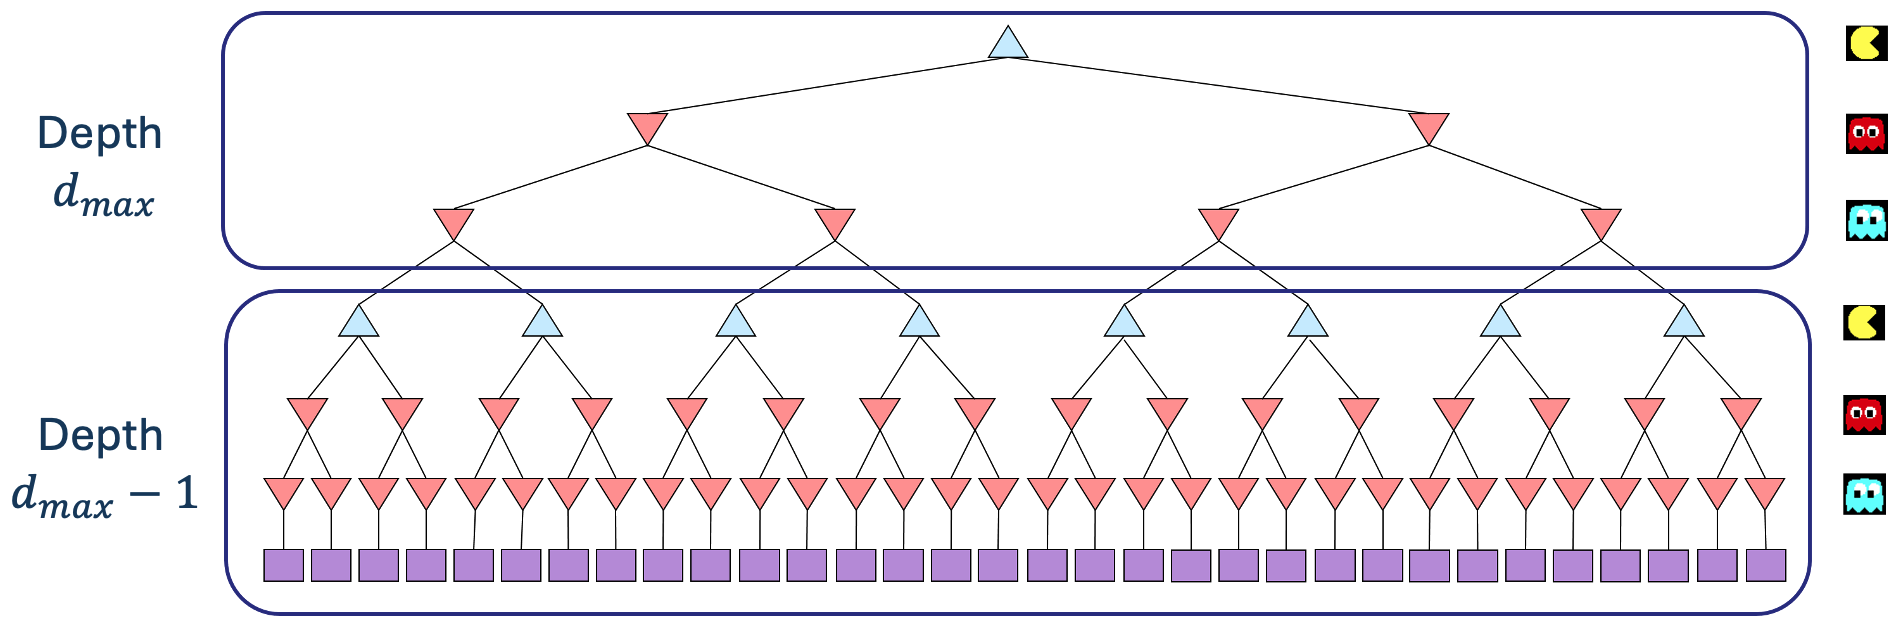
\includegraphics[width=0.75\linewidth]{05_pacman/minimax_depth.png}
  \caption{Depth vs.\ tree height (from the handout).}
\end{figure}
\expect{The recurrence as a piecewise function, using exactly these functions.}
\begin{solution}
\[
V_{\text{minmax}}(s,d)=
\begin{cases}
\text{Utility}(s) & \text{IsEnd}(s)\\
\todo{} & \todo{}\\
\end{cases}
\]
\end{solution}

\problempart{1b}{\texttt{MinimaxAgent}}
\codepart{5.1b}

% ----------------------------------------------------------------------------
\subsection{Alpha-beta pruning}
\codepart{5.2a}

% ----------------------------------------------------------------------------
\subsection{Expectimax}

\problempart{3a}{Expectimax recurrence}
\question{Write $V_{\text{exptmax}}(s,d)$, the maximum expected utility against ghosts that each pick a legal move
uniformly at random, using the same functions as in 1a.}
\expect{A piecewise recurrence in the style of 1a.}
\begin{solution}
\todo{answer}
\end{solution}

\problempart{3b}{\texttt{ExpectimaxAgent}}
\codepart{5.3b}

% ----------------------------------------------------------------------------
\subsection{Evaluation function (extra credit)}

\problempart{4a}{\texttt{better\_evaluation\_function}}
\codepart{5.4a}

\problempart{4b}{Describing the evaluation function}
\question{Describe the evaluation function and its high-level motivation. What else did you try, and what worked
and what did not? State whether you consent to the solution being shared if it places in the top 3.}
\expect{A short paragraph.}
\begin{solution}
\todo{answer}
\end{solution}

% ----------------------------------------------------------------------------
\subsection{AI (mis)alignment and reward hacking}

Compare \texttt{python pacman.py -p MinimaxAgent -l trappedClassic -a depth=3} with the
\texttt{ExpectimaxAgent} on the same layout (run each several times).

\problempart{5a}{Why the agents differ}
\question{Why does the minimax agent always rush towards the \emph{closest} ghost, while the expectimax agent
(occasionally) does not?}
\expect{One sentence for minimax, stating the assumption that causes this, and one sentence for expectimax.}
\begin{solution}
\todo{answer}
\end{solution}

\problempart{5b}{Fixing the objective}
\question{Suggest a change to $\text{Eval}(s)$ (\texttt{score\_evaluation\_function}) and/or $\text{Utility}(s)$ (the
final score), or to how the game score is computed, that would stop minimax from dying instantly on
\texttt{trappedClassic} and make it behave more like expectimax.}
\expect{1--2 sentences describing the change and why it works.}
\begin{solution}
\todo{answer}
\end{solution}

\problempart{5c}{Another real-world example}
\question{Describe a realistic scenario outside Pac-Man in which a designer's objective is open to reward hacking
or causes negative side effects.}
\expect{2--5 sentences, stating whether it is reward hacking, a negative side effect, or both, with a justification.}
\begin{solution}
\todo{answer}
\end{solution}
